% generated by experiments/build_paper_assets.py -- do not edit by hand
\begin{figure}[t]
\centering
\resizebox{\linewidth}{!}{%
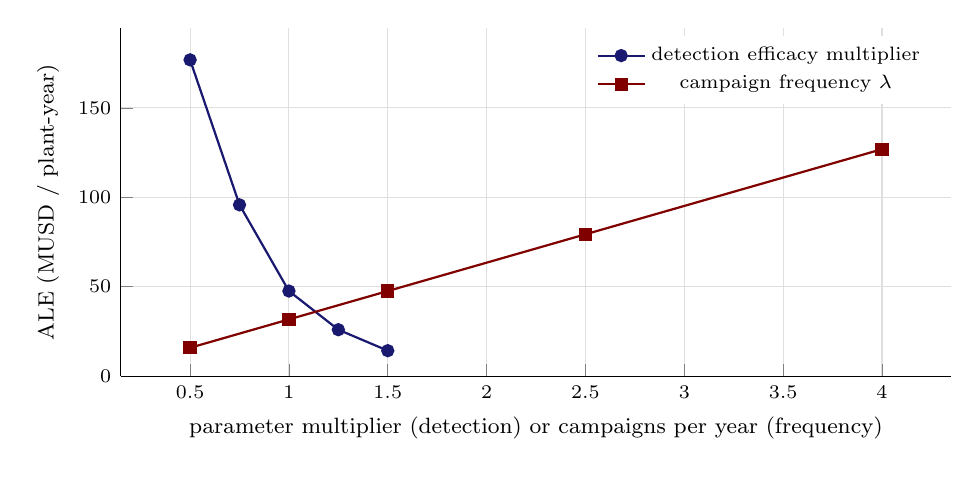
\begin{tikzpicture}
\begin{axis}[
    width=\linewidth, height=6.0cm,
    xlabel={parameter multiplier (detection) or campaigns per year (frequency)},
    ylabel={ALE (MUSD / plant-year)},
    ymin=0, legend style={at={(0.98,0.98)}, anchor=north east, font=\scriptsize, draw=none},
    ticklabel style={font=\scriptsize}, label style={font=\footnotesize},
    xmajorgrids, ymajorgrids, grid style={gray!25}, axis lines*=left,
]
\addplot[MidnightBlue, thick, mark=*] coordinates {(0.5,176.803) (0.75,95.751) (1.0,47.567) (1.25,25.945) (1.5,14.228)};
\addplot[Maroon, thick, mark=square*] coordinates {(0.5,15.856) (1.0,31.712) (1.5,47.567) (2.5,79.279) (4.0,126.846)};
\legend{detection efficacy multiplier, campaign frequency $\lambda$}
\end{axis}
\end{tikzpicture}}
\caption{One-at-a-time sensitivity of the annualised loss expectancy. Halving detection efficacy multiplies the baseline ALE by 3.7; the response to campaign frequency is linear by construction.}
\label{fig:sensitivity}
\end{figure}
